\documentclass[\main.tex]{subfiles}

\chapter{Metodologia de Operacionalização do Trabalho}

\section{Processo e Metodologia de Trabalho}
Foi adotada uma abordagem iterativa incremental, com algumas reuniões de acompanhamento ao
longo do projeto. No decorrer de 15 semanas, foram criadas 4 iterações pelas quais foram
divididas as tarefas em cima descritas.\par
O \textit{\gls{roadmap}} do projeto, que se encontra representado na forma de um diagrama de
Gantt, apresenta, mais detalhadamente, a atribuição das tarefas nas diferentes iterações e a
duração das mesmas.
\vspace{5pt}

\begin{figure}[h]
\centering
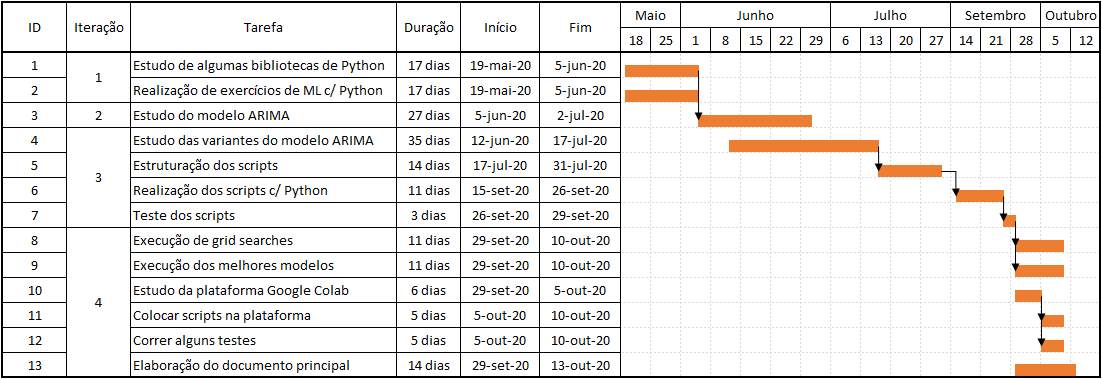
\includegraphics[width=\linewidth]{../private_assets/Roadmap.png}
\caption{Diagrama de Gantt representativo do \textit{\gls{roadmap}} do projeto}
\end{figure}


\newpage
\section{Arquitetura Concetual}
A arquitetura da plataforma de testes está representada na figura 3.2.\par

\begin{figure}[h!]
\centering
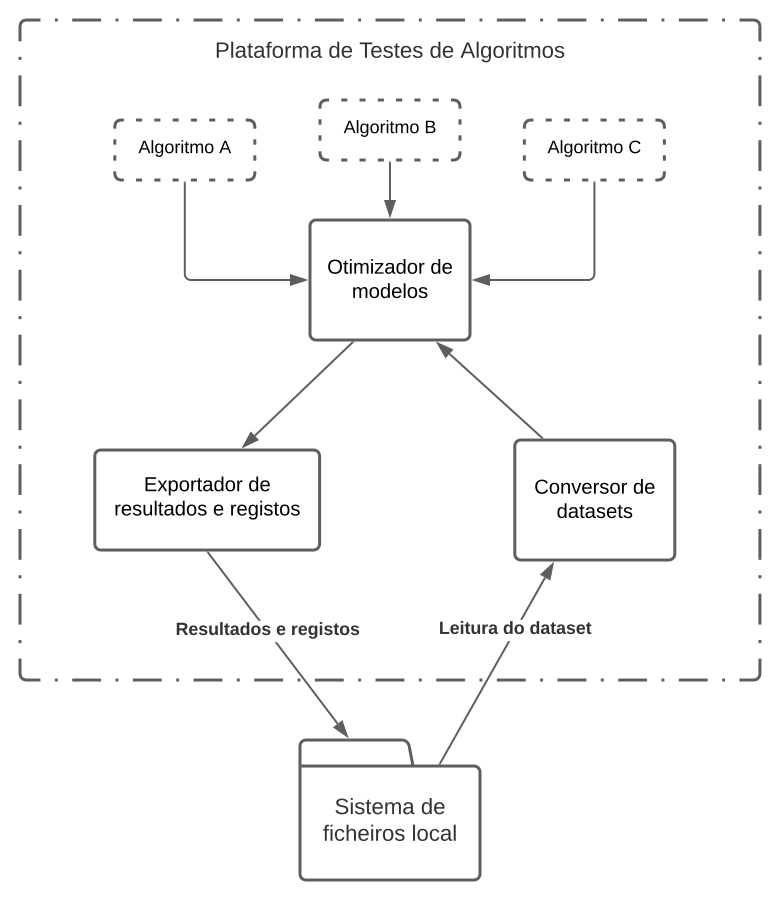
\includegraphics[width=0.8\linewidth]{../private_assets/Arquitetura_App.png}
\caption{Arquitetura da aplicação}
\end{figure}\par

Na \acrfull{poo}, o encapsulamento refere-se ao agrupamento de dados com os métodos que
operam nesses dados ou à restrição do acesso direto a alguns dos componentes de um objeto.
\cite{encapsulation_paul_rogers} O encapsulamento é utilizado para ocultar os valores ou o
estado de um objeto de dados estruturados dentro de uma classe, evitando o acesso direto de
terceiros não autorizados a eles.\par
Este mecanismo não é exclusivo para \acrshort{poo}. Implementação de dados abstratos, como
por exemplo módulos, oferecem uma forma semelhante de encapsulamento. A similaridade foi
explicada por teóricos da linguagem de programação em termos de tipos existenciais.
\cite{data_abstraction_existentials}\par
Para a realização deste projeto foi necessário a utilização de encapsulamento, de modo a
manter uma boa estrutura e organização do código.\par
Em relação à estrura das pesquisas em grelha, foram todas desenhadas e pensadas à medida do
projeto, a fim de testar o maior número possível de modelos para um determinado
\textit{\gls{dataset}}.
\enlargethispage{\baselineskip}

\section{Desenvolvimento da Solução}
Tal como está descrito na arquitetura concetual do projeto, foi necessário
desenvolver 3 componentes principais: um conversor de \textit{\glspl{dataset}} para
transformar o conjunto de dados armazenado no sistema de ficheiros num objeto
\textit{\say{DataFrame}} da biblioteca \textit{pandas}; um corredor de modelos, que permite
correr todos os modelos para o dataset carregado anteriormente; um exportador de resultados
e registos, isto é, os resultados (tempo de execução, \textit{\acrshort{mae}},
\textit{\acrshort{mse}}, \textit{\acrshort{rmse}}) serão exportado para um ficheiro
\textit{.csv}. Os registos são as mensagens de sucesso ou erro apresentadas no final de cada
modelo, que serão exportadas para um ficheiro \textit{.txt}. A figura 4.3 representa o
diagrama de classes das entidades elaboradas.

\begin{figure}[h!]
\centering
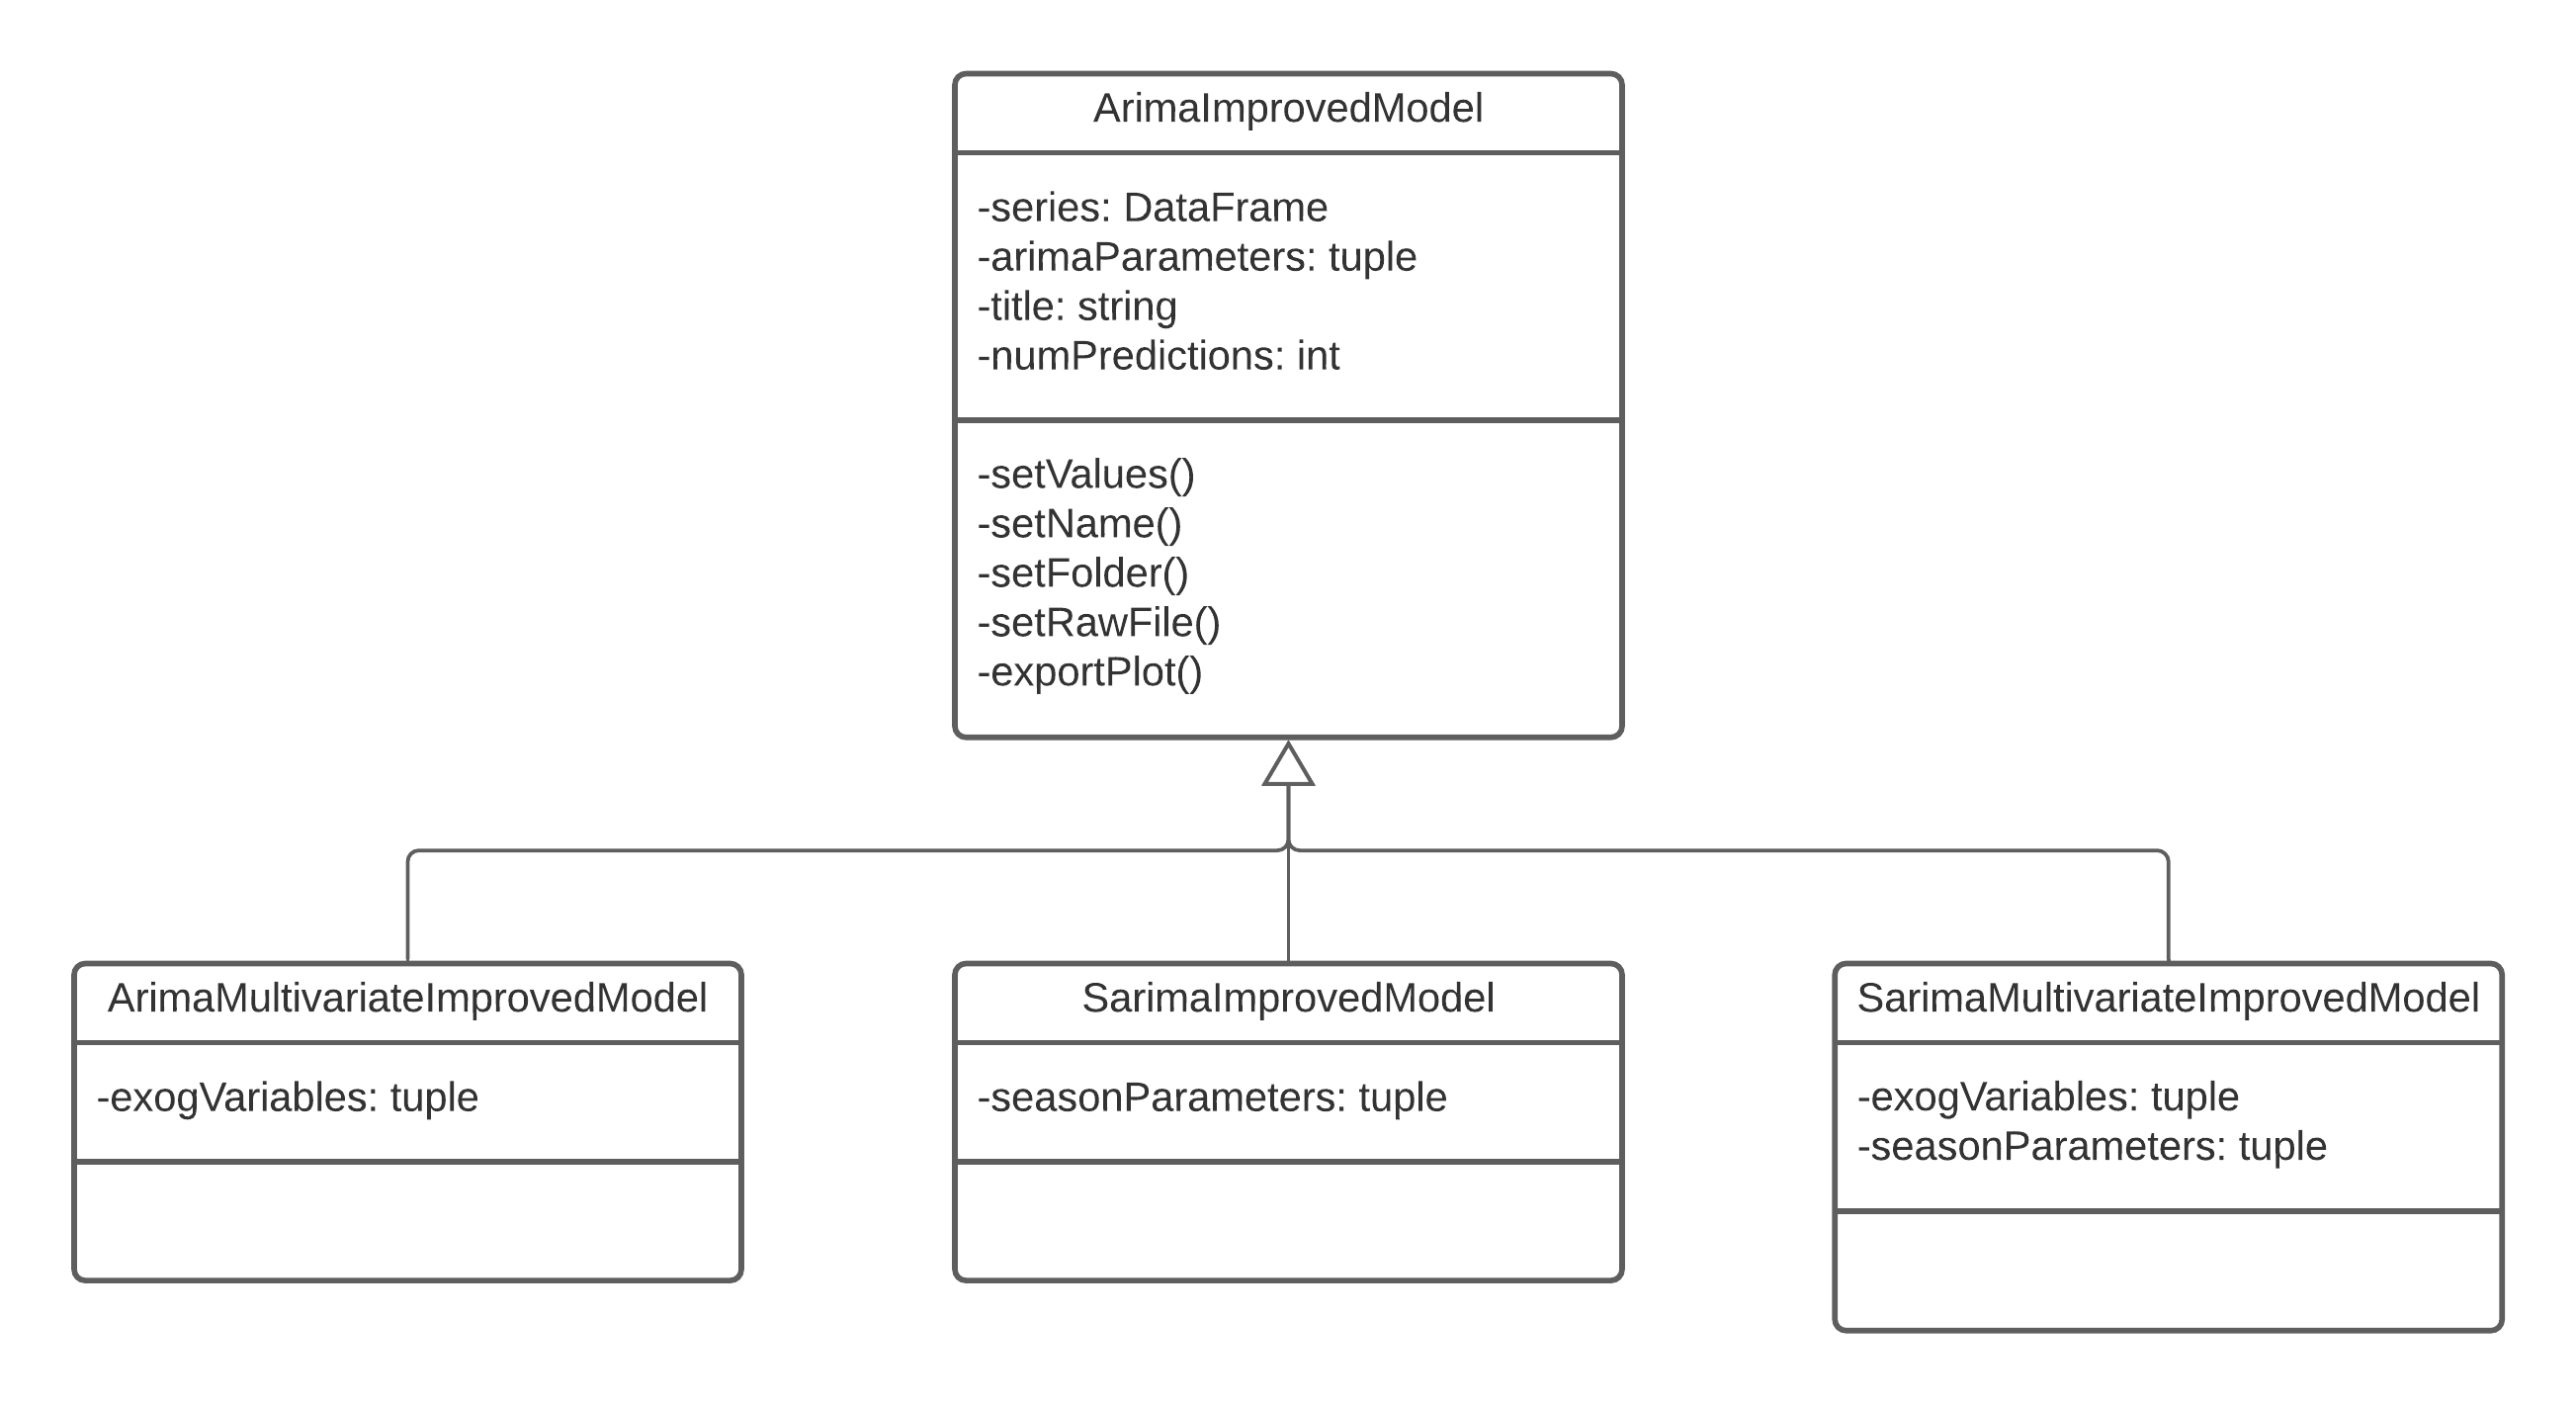
\includegraphics[width=\linewidth]{../private_assets/ClassDiagram_App.png}
\caption{Diagrama de classes do projeto}
\end{figure}\par


\subsection{Conversor de \textit{datasets}}
Primeiramente, temos o conversor de \textit{\glspl{dataset}}. No excerto de código 4.1,
pode ser analisado este componente.\par
\vspace{10pt}

\begin{lstlisting}[language=Python, caption=Componente de conversão de \textit{datasets}]
def _dataset_to_series(filename: str, date_parser=None):
    """Searches FILES_FOLDER for a dataset and returns it into a DataFrame
    object. If it is needed to parse the dates, a function should be passed
    as the "date_parser" argument.

    Args:
        filename (str): name of the .csv file containing the dataset. This file
            should be in the FILES_FOLDER.
        date_parser (optional): function to parse the dates of the dataset if
            needed. The function should return a datetime.
    """
    FILES_FOLDER = "datasets"
    file_path = os.path.join(FILES_FOLDER, filename)
    series = DataFrame()
    try:
        series = read_csv(file_path, header=0, index_col=0, parse_dates=[0],
                          infer_datetime_format=True, date_parser=date_parser)
    except Exception as err:
        print(f"('{filename}') {type(err).__name__}: {err}")
    return series
\end{lstlisting}\par
Depois de analisar este excerto de código, podemos concluir que este não é dos componentes
mais complexos, porém, exige uma compreensão mínima da biblioteca (\textit{pandas}), visto
que caso seja necessário realizar alguma alteração nalgum parâmetro para converter o
\textit{\gls{dataset}}, deve ser feito com cautela e alguma investigação do método
\textit{\say{read\_csv()}}.\par
Concluindo, este método faz a leitura de um ficheiro no diretório \textit{\say{datasets}}
e faz a conversão do mesmo para um objeto \textit{\say{DataFrame}}, a fim de ser utilizado
pelos próximos componentes.


\subsection{Exportador de resultados e registos}
O excerto de código 4.2 é representativo do componente exportador de resultados e registos.
\vspace{10pt}

\begin{lstlisting}[language=Python, caption=Componente de exporte de resultados e registos]
def _export_results(results_order: str = "name"):
    """Exports the results list into a .csv file ordered by the model order

    Args:
        results_order (str): order factor of the results list. ("name", "time",
            "mae", "mse" or "rmse"). Defaults to "name".
    """
    order = results_order.lower()
    if order == "time":
        order_num = 1
        order_name = "Execution Time (sec)"
    elif order == "mae":
        order_num = 2
        order_name = "MAE"
    elif order == "mse":
        order_num = 3
        order_name = "MSE"
    elif order == "rmse":
        order_num = 2
        order_name = "RMSE"
    else:
        order_num = 0
        order_name = "Model Name"

    results.sort(key=lambda line: float(line[order_num]))

    results_file = CSVWriter(
                       os.path.join(OUTPUT_FOLDER, "results_summary.csv"),
                       ("Model", "Execution Time (sec)", "MAE", "MSE", "RMSE")
                   )
    results_file.write_at_once(results)
    results_file.close()

    print(f"Results list file finished. Ordered by {order_name}.")


def _export_logs():
    """Exports the log list into a .txt file"""
    log_file = open(os.path.join(OUTPUT_FOLDER, "log.txt"), "w")
    for log in logs:
        log_file.write(log)
        log_file.write("\n")
    log_file.close()
    print("Log file finished.")

\end{lstlisting}\par

Neste componente, podemos visualizar a existência de duas funções. A primeira é destinada a
exportar os resultados de todos os modelos corridos pela aplicação ordenados pelo nome,
pelo \textit{\acrshort{mae}}, \textit{\acrshort{mse}} ou pelo \textit{\acrshort{rmse}}.
Todos os modelos que não tiveram sucesso na sua execução terão os seus erros todos com o
valor de \say{-1}, visto que é um valor impossível de obter se o modelo tiver terminado
com sucesso.\par
Em relação à função de exportar os registos, trata-se de um subcomponente informativo, dado
que não tem nenhuma utilidade prática para o sucesso ou insucesso dos modelos, mas apenas
para informar que modelos tiveram sucesso e quais os que não tiveram e porquê.



\subsection{Corredor de modelos}
O excerto de código 4.3 representa o componente realizado para correr os modelos.\par
\vspace{10pt}

\begin{lstlisting}[language=Python, caption=Componente para correr os modelos]
def run_models(dataset_name: str, models: list, variable_to_predict: str,
                   title: str, results_order: str, num_splits: int = 0,
                   num_predictions: int = 10, predictions_size: float = 0,
                   date_parser=None):
    """Parses the dataset (.csv file) into a DataFrame object and runs ARIMA
    models with the given dataset.

    Args:
        dataset_name (str): name of the .csv file with the dataset.
        models (list): list of dictionaries with the ARIMA models to be tested.
        title (str): title to be used in the output files to distinguish the
            models.
        variable_to_predict (str): name of the variable to predict. It must be
            the same name of the column in the dataset.
        results_order (str): order factor of the results list. ("name", "time",
            "mae", "mse" or "rmse").
        num_splits (int): number of splits in case of being cross validation
            models. Defaults to 0.
        num_predictions (int): number of predictions of the model. Defaults
            to 10. It will only have effect if the predictions_size is equal
            to zero.
        predictions_size (float): percentage of data to predict (from 0 to 1).
            Defaults to 0.
        date_parser (optional): function to parse the dates of the dataset if 
            needed. The function should return a datetime.
    """
    series = _dataset_to_series(dataset_name, date_parser)

    for model in models:
        for arima_parameters in model.get("arima_parameters"):
            if model.get("model") == ArimaImprovedModel:
                model.get("model")(series=series,
                                   variable_to_predict=variable_to_predict,
                                   arima_parameters=arima_parameters,
                                   num_predictions=num_predictions,
                                   predictions_size=predictions_size,
                                   title=title,
                                   num_splits=num_splits)
            elif model.get("model") == ArimaMultivariateImprovedModel:
                exog_variables = model.get("exog_variables")
                model.get("model")(series=series,
                                   variable_to_predict=variable_to_predict,
                                   exog_variables=exog_variables,
                                   arima_parameters=arima_parameters,
                                   num_predictions=num_predictions,
                                   predictions_size=predictions_size,
                                   title=title,
                                   num_splits=num_splits)
            elif model.get("model") == SarimaImprovedModel:
                for season_parameters in model.get("season_parameters"):
                    model.get("model")(series=series,
                                       variable_to_predict=variable_to_predict,
                                       arima_parameters=arima_parameters,
                                       season_parameters=season_parameters,
                                       num_predictions=num_predictions,
                                       predictions_size=predictions_size,
                                       title=title,
                                       num_splits=num_splits)
            elif model.get("model") == SarimaMultivariateImprovedModel:
                exog_variables = model.get("exog_variables")
                for season_parameters in model.get("season_parameters"):
                    model.get("model")(series=series,
                    variable_to_predict=variable_to_predict,
                                       exog_variables=exog_variables,
                                       arima_parameters=arima_parameters,
                                       season_parameters=season_parameters,
                                       num_predictions=num_predictions,
                                       predictions_size=predictions_size,
                                       title=title,
                                       num_splits=num_splits)
            else:
                logs.append(f"LOG: Model {model.get('model')} was not found!")
    _export_results(results_order)
    _export_logs()
\end{lstlisting}\par

Este é possivelmente o componente mais minucioso e onde mais erros podem acontecer, visto
que se trata do componente \textit{\say{core}}. Neste componente são chamados os outros
dois anteriores. Este é, provavelmente, o componente que seria servido, caso fosse criada
uma \textit{\acrshort{api}} no final do desenvolvimento do projeto. Esta função percorre
a lista de modelos e recebe a série temporal, para puder tratar de fazer as previsões,
guardando o resumo do desempenho de cada modelo num \textit{array} e os registos de cada
modelo noutro. À medida que cada modelo termina, os resultados e o seu registo são anexados
às respetivas listas. Também pode-se ir vendo os diretórios a serem criados à medida que 
os modelos terminam (desde que terminem com sucesso, caso contrário, como não há resultados,
a pasta é apagada). No final, são criados o ficheiro de resumo dos resultados e o ficheiro
de registos.\par

\subsection{Função \textit{init()}}
A função \textit{init()} serve para testar implementações de código e fazer demonstrações
do mesmo. No excerto 4.4 está representada esta mesma função, que demonstra a forma como
devem ser instanciados e executados os modelos de aprendizagem.

\begin{lstlisting}[language=Python, caption=Função init]
    def init():
    dataset = "LinkNYC_kiosk.csv"

    def parser(x):
        return datetime.strptime(x, "%d/%m/%Y")

    variable_to_predict = "census"

    arima_parameters = [(1, 2, 0), (3, 2, 0), (2, 2, 0), (4, 2, 0)]

    sarima_parameters = [(1, 2, 0, 24), (1, 2, 0, 168)]

    exog_variables = ("temp", "heating degree", "cooling degree")

    models = [
        {
            "model": ArimaImprovedModel,
            "arima_parameters": arima_parameters
        },
        {
            "model": ArimaMultivariateImprovedModel,
            "arima_parameters": arima_parameters,
            "exog_variables": exog_variables
        },
        {
            "model": SarimaImprovedModel,
            "arima_parameters": arima_parameters,
            "season_parameters": sarima_parameters
        },
        {
            "model": SarimaMultivariateImprovedModel,
            "arima_parameters": arima_parameters,
            "exog_variables": exog_variables,
            "season_parameters": sarima_parameters
        }
    ]

    num_predictions = 20

    title = "Census"

    num_splits = 3

    results_order = "mse"

    run_models(dataset_name=dataset,
               variable_to_predict=variable_to_predict,
               date_parser=parser,
               models=models,
               num_predictions=num_predictions,
               title=title,
               num_splits=num_splits,
               results_order=results_order)
\end{lstlisting}


\subsection{\textit{ARIMA} class}
O modelo \textit{\gls{arima}} está representado no código através da classe
\textit{ArimaImprovedModel}. Esta classe está representada no excerto de código 4.5.\par

\subsection{\textit{ARIMAX} class}
O modelo \textit{\gls{arimax}} está representado no código através da classe
\textit{ArimaMultivariateImprovedModel}. Esta classe está representada no excerto de
código 4.6.\par

\subsection{\textit{SARIMA} class}
O modelo \textit{\gls{sarima}} está representado no código através da classe
\textit{SarimaImprovedModel}. Esta classe está representada no excerto de código 4.7.\par

\subsection{\textit{SARIMAX} class}
O modelo \textit{\gls{sarimax}} está representado no código através da classe
\textit{SarimaMultivariateImprovedModel}. Esta classe está representada no excerto de
código 4.8.\par

\newpage